% !TeX root = ../documento.tex
\chapter{Metodologia}
\label{chap:metodologia}
A presente pesquisa procura analisar estratégias de controle digital aplicadas a sistemas de frenagem automotiva, com ênfase em aplicações de Controle de Cruzeiro Adaptativo (ACC). Para isso, foi desenvolvida uma plataforma experimental que permite a coleta de dados de sensores e o acionamento de atuadores relevantes ao sistema de freio. 
% O estudo se concentra na modelagem, simulação e validação do comportamento do sistema em situações de frenagem, utilizando o ambiente Matlab/Simulink para a implementação e avaliação dos algoritmos de controle.

O estudo se concentra na modelagem e simulação do comportamento hidráulico do sistema de frenagem, bem como na avaliação, em ambiente controlado, das estratégias de controle digital responsáveis pela modulação de pressão. O ambiente Matlab/Simulink é utilizado para representar matematicamente o sistema e implementar os algoritmos de controle que são posteriormente validados frente a cenários típicos de frenagem.

A escolha dos componentes eletrônicos e do microcontrolador, como os circuitos integrados MC34SB0410AE, MC34SB0800AE e o AURIX TC375, foi orientada por critérios de viabilidade experimental e compatibilidade com as demandas de simulação e controle digital. Esses elementos viabilizam a realização dos experimentos propostos, mas não constituem o foco central da investigação.

%É importante destacar que o escopo deste trabalho está restrito à validação do sistema em ambiente simulado e controlado, reconhecendo-se limitações inerentes à experimentação laboratorial e à modelagem adotada.

É importante destacar que o escopo deste trabalho está principalmente orientado à validação dos modelos e das estratégias de controle em ambiente simulado, ainda que a plataforma experimental desenvolvida permita a aquisição de sinais reais. Dessa forma, reconhecem‑se as limitações inerentes à experimentação laboratorial e às simplificações adotadas na modelagem. Os resultados obtidos devem ser interpretados como subsídio para pesquisas e aprimoramentos futuros, especialmente no contexto de aplicações em veículos autônomos e sistemas ADAS.

Este capítulo está organizado para apresentar, inicialmente, a modelagem matemática do sistema de frenagem automotivo, destacando os principais elementos dinâmicos envolvidos. Em seguida, são descritos os modelos implementados no ambiente Matlab/Simulink e as estratégias de controle digital adotadas. Por fim, são apresentados os cenários de simulação e os critérios utilizados para a validação dos resultados, evidenciando a relação entre o modelo teórico, sua implementação computacional e a análise do desempenho do sistema.

% ADD 01/29/2026 (movido para arquivo separado)
% !TeX root = ../documento.tex

% Conteúdo extraído de elementos-textuais/metodologia.tex para manter o arquivo principal mais enxuto.

\section{Procedimento metodológico e métricas de avaliação}
\label{sec:metodologia-procedimento}

O procedimento adotado neste trabalho segue o fluxo: (i) modelagem do subsistema hidráulico de freio, (ii) linearização em torno de um ponto de operação, (iii) projeto do controlador (LQI) e do observador (Luenberger), (iv) implementação digital no ambiente MATLAB/Simulink e (v) validação por simulação em malha aberta e em malha fechada.

Para evitar que o texto principal assuma a forma de um “manual de MATLAB”, a descrição do uso de \textit{scripts} é feita de maneira conceitual: no corpo do texto, explicita-se o papel do \textit{script} na organização do ensaio (definição do horizonte de simulação, parametrização do modelo, geração de comandos/referências e registro de sinais); já o detalhe de implementação (funções, variáveis e trechos de código) é apresentado no apêndice de códigos.

As métricas de avaliação foram escolhidas para refletir tanto desempenho de seguimento quanto esforço de atuação: tempo de subida e de acomodação da pressão, sobressinal, erro de regime permanente e erro RMS. Complementarmente, registra-se o esforço máximo de controle (por exemplo, máximos de $u_{in}$ e $u_{out}$) para verificar compatibilidade com as saturações físicas impostas no modelo. A apresentação dos resultados (curvas, métricas e discussão) é concentrada no Capítulo~\ref{chap:resultados}, de modo que a metodologia permaneça claramente separada dos achados.
% END ADD

\section{Tipo e Abordagem da Pesquisa}
\label{sec:metodologia-1}
A pesquisa adotada é computacional, uma vez que utiliza modelos matemáticos, simulações e algoritmos para analisar o desempenho do sistema em ambiente MATLAB/Simulink. Em paralelo, é desenvolvido um protótipo de plataforma eletrônica como suporte à futura migração do controlador para execução embarcada.


\section{Justificativa das Escolhas Metodológicas}
\label{sec:metodologia-2}
As escolhas metodológicas adotadas neste trabalho foram fundamentadas em referências da literatura e na necessidade de validar, em simulação, estratégias de controle digital para sistemas de freio automotivo, ao mesmo tempo em que se estrutura a migração para validação experimental em etapas futuras. A seleção dos componentes, algoritmos e procedimentos buscou responder certas lacunas identificadas em projetos anteriores, garantindo rigor científico e relevância para futuras pesquisas.


\section{Aplicação em ADAS}
\label{sec:metodologia-3}

Os sistemas ADAS são projetados especialmente para aumentar a segurança e a eficiência dos veículos, utilizando uma combinação de sensores e tecnologias de controle. Esse conjunto de elementos interligados é capaz de monitorar o ambiente ao redor do veículo e tomar decisões em tempo real para auxiliar o motorista em diversas situações de condução. 

A integração do sistema de freio com controle digital em um ambiente controlado, aliado à arquitetura de um veículo equipado com (ADAS), possibilita uma análise mais precisa e eficiente do comportamento do sistema durante a frenagem. Essa abordagem favorece a coleta de dados relevantes para a avaliação da segurança e do desempenho em diferentes cenários.

De acordo com \citeonline{Lentin2022}, um veículo com arquitetura ADAS possui como principais interfaces: câmeras, LIDARs, RADARs, SONARs, \gls{IMU} e receptores \gls{GNSS} para analisar o ambiente e tomar decisões adequadas para atuação. Ele ainda descreve que, no contexto de um veículo com ADAS, o sistema de controle é dedicado à geração de comandos apropriados para o acelerador, freio e direção, a fim de executar um movimento controlado.

\subsection{Integração com ADAS}
\label{sebsec:metodologia-3-1}
No contexto deste estudo, a integração do sistema de controle digital de frenagem com sistemas avançados de assistência ao condutor ADAS é analisada a partir de casos de uso específicos, com foco em aplicações de controle longitudinal veicular. Em particular, considera-se a atuação do sistema de frenagem no âmbito do Adaptive Cruise Control (ACC), funcionalidade amplamente presente em veículos modernos e fortemente dependente da modulação precisa da pressão de freio.

Os cenários analisados são inspirados em manobras padronizadas utilizadas por protocolos de avaliação de segurança veicular, como os ensaios propostos pelo EuroNCAP, que envolvem situações de aproximação de um veículo à frente e necessidade de redução controlada da velocidade. Nesses cenários, os sistemas ADAS utilizam informações provenientes de sensores como radar e câmera para estimar a distância relativa e a velocidade dos obstáculos, gerando, a partir de seus algoritmos de decisão, uma referência de desaceleração longitudinal.

Nesse contexto, o sistema de frenagem modelado neste trabalho atua como o estágio final da cadeia de controle, sendo responsável por converter a demanda de desaceleração fornecida pelo módulo ADAS em pressão hidráulica efetiva nos atuadores de freio. O estudo concentra-se, portanto, na dinâmica da geração de pressão por meio da bomba hidráulica, assumindo válvulas em estados discretos (abertas ou fechadas), para isolar e analisar o impacto da atuação da bomba sobre a resposta do sistema.

A adoção desse recorte permite avaliar, em ambiente controlado, o comportamento dinâmico do sistema de frenagem diante de comandos típicos de ADAS, como variações abruptas ou graduais da demanda de frenagem. Dessa forma, contribui-se para a compreensão dos desafios associados à integração entre algoritmos de assistência à condução e sistemas hidráulicos de freio, mantendo o foco nos aspectos fundamentais da modelagem e do controle da pressão.

\section{Descrição do Sistema de Freio}
\label{sec:metodologia-4}

O sistema de freio automotivo veicular conhecido atualmente \cite{Konrad2014}, é composto por um pedal do freio (1), o servofreio (2), o cilindro mestre (3), o reservatório (4), as linhas de freio, (5) as mangueiras (6) e os freios e cilindros de freio de roda (7). Há também os seguintes componentes que vão ter destaque durante o desenvolvimento do projeto: os sensores de velocidade da roda (8), o bloco hidráulico (9) e a unidade de controle (10), como mostra a Figura~\ref{fig:sistema-de-freio-com-abs}.

Embora essa arquitetura inclua o caminho tradicional de geração de pressão por meio do cilindro mestre (associado ao pedal), o recorte deste trabalho concentra-se no uso do conjunto eletro-hidráulico (unidade ABS/ESC: bomba, válvulas e eletrônica) como \textbf{atuador de pressão em frenagem ativa}, isto é, com referência de pressão proveniente de uma função ADAS longitudinal (por exemplo, ACC/AEB), conforme discutido na Seção~\ref{sec:metodologia-3}. Nesse modo de operação, a pressão pode ser gerada/recomposta pela bomba e modulada por válvulas por canal, podendo haver isolamento hidráulico do cilindro mestre, dependendo da arquitetura do sistema.


\begin{figure}[htbp]
    \centering
    \caption{Sistema de Freio}
    \label{fig:sistema-de-freio-com-abs}
    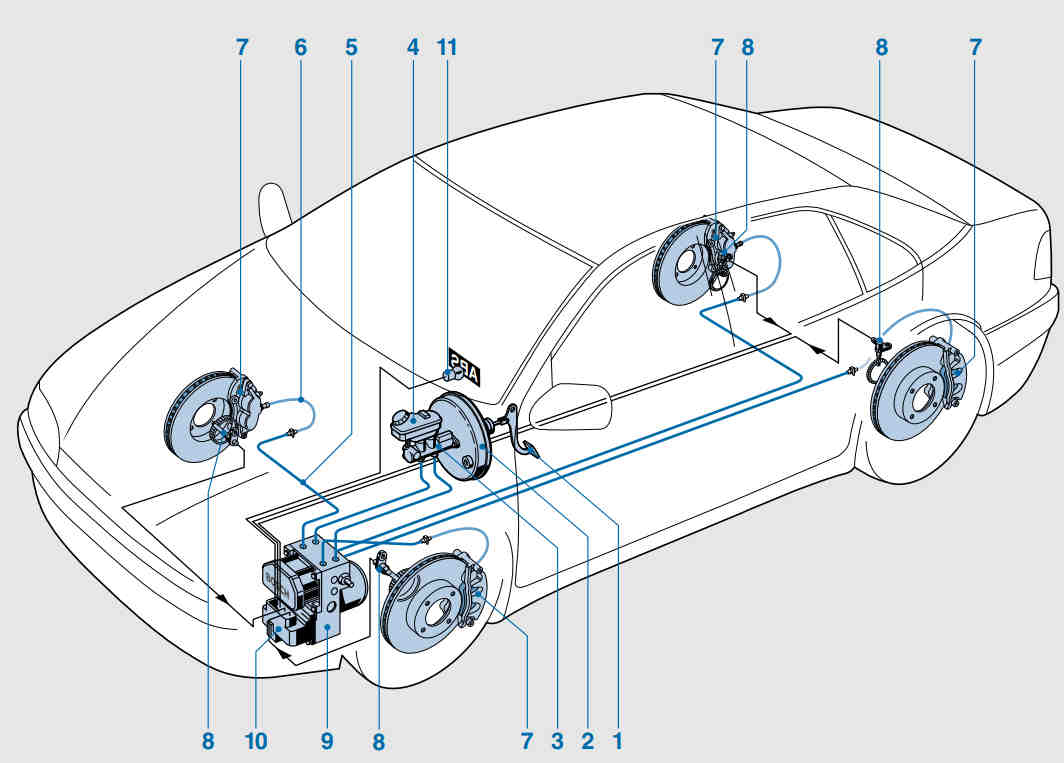
\includegraphics[width=0.8\textwidth]{figuras/sistema-de-freio-com-abs.jpg}
    \fonte{ O Autor, adaptado de \cite{Konrad2014}.}
\end{figure}


Outra parte a ser destacada desse sistema é a parte hidráulica, responsável por conduzir o fluido de freio para exercer pressão na pastilha contra o disco. O uso de sistemas eletro-hidráulicos, especialmente em veículos elétricos, tem sido objeto de estudos recentes que visam otimizar o desempenho do motor e do sistema de frenagem de forma integrada \cite{MotorParametricDesign2023}.

 \begin{figure}[htbp]
    \centering
    \caption{Princípio do Bloco Hidráulico com Válvulas Solenoides}
    \label{fig:principio-do-modulador-hidraulico-com-valvulas-solenoides}
    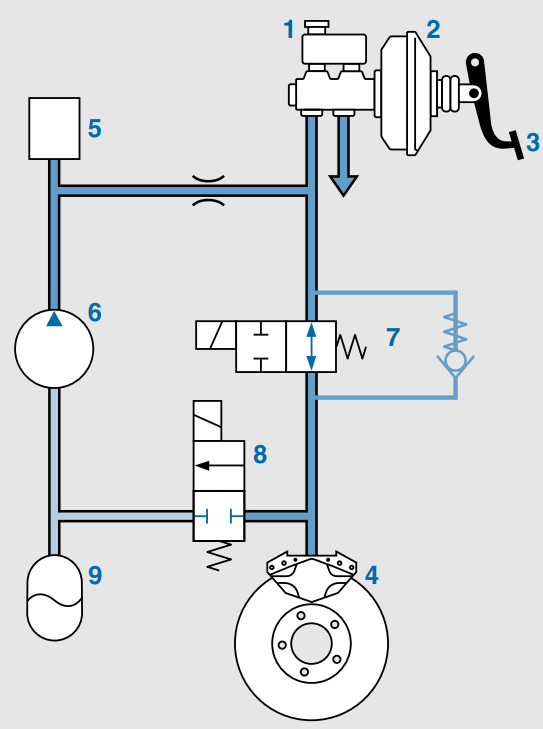
\includegraphics[width=0.8\textwidth]{figuras/principio-do-modulador-hidraulico-com-valvulas-solenoides.png}
    \fonte{ O Autor, adaptado de \cite{Konrad2014}.}
\end{figure}

 
O bloco hidráulico incorpora múltiplas válvulas solenoides que abrem ou fecham caminhos hidráulicos entre o cilindro mestre/suprimento, o retorno e os canais de roda, como mostra a Figura~\ref{fig:principio-do-modulador-hidraulico-com-valvulas-solenoides}. 

%Ele também conecta os freios à bomba de retorno (6). Válvulas solenoides com duas conexões hidráulicas e duas posições de válvula são usadas (válvulas solenoides 2/2). A válvula de entrada (7), entre o cilindro mestre e o freio, controla a aplicação de pressão, enquanto a válvula de saída (8), entre o freio e a bomba de retorno, controla a liberação de pressão. Há um par de válvulas solenoides para cada freio.

Ele também conecta os freios à bomba de retorno (6). Válvulas solenoides com duas conexões hidráulicas e duas posições de válvula são usadas (válvulas solenoides 2/2). A válvula de entrada (7), entre o cilindro mestre e o freio, controla a vazão de entrada de fluido para o circuito de freio, enquanto a válvula de saída (8), entre o freio e a bomba de retorno, controla a \textbf{vazão de saída} do fluido para o reservatório de baixa pressão. Há um par de válvulas solenoides para cada freio.


\subsection{Válvulas Solenoide}
\label{sec:metodologia-4-1}

As válvulas são indispensáveis, porque modulam a pressão do sistema.
A Figura~\ref{fig:modelo-hidraulico-conjunto-freio} apresenta o modelo hidráulico com o conjunto de freio automotivo.

 \begin{figure}[htbp]
    \centering
    \caption{Modelo Hidráulico com Conjunto de Freio Automotivo.}
    \label{fig:modelo-hidraulico-conjunto-freio}
    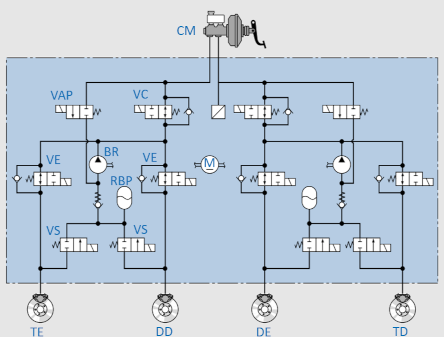
\includegraphics[width=0.8\textwidth]{figuras/modelo-hidraulico-conjunto-freio.png}
    \fonte{ O Autor, adaptado de \cite{Konrad2014}.}
\end{figure}

O processo de modulação hidráulica em unidades ABS/ESC pode ser descrito, de forma funcional, pelos três modos clássicos de atuação no canal/roda: \textit{aumento de pressão} (pressurização), \textit{retenção} (\textit{hold}) e \textit{redução de pressão} (alívio). Em termos hidráulicos, esses modos decorrem da combinação de estados das válvulas de entrada (que estabelecem ou bloqueiam a comunicação com o suprimento) e de saída (que estabelecem ou bloqueiam a comunicação com o retorno), bem como do acionamento do conjunto motor+bomba.

No \textbf{ABS clássico} (frenagem comandada pelo condutor), a pressão base é gerada no cilindro mestre e a unidade hidráulica atua modulando-a por roda, tipicamente com recirculação para recomposição de pressão. Já em \textbf{frenagem ativa} (ESC/ADAS), a unidade eletro-hidráulica pode assumir o papel de atuador principal de pressão, impondo perfis de pressão por roda a partir de uma referência gerada eletronicamente. Esse é o modo de interesse deste trabalho.

\subsection{Motor da Bomba de Pressão}
\label{sec:metodologia-4-2}
A função do conjunto motor+bomba é fornecer vazão ao suprimento e permitir a recomposição/geração de pressão hidráulica necessária para a modulação por canal. Em ABS/ESC, esse conjunto pode operar tanto para recirculação (recomposição durante modulação) quanto, em arquiteturas de frenagem ativa, como fonte primária de pressão para impor perfis de pressão por roda.

%A bomba normalmente consiste em um motor, geralmente BLDC (que significa \textit{Brushless Direct Current}, que se traduz para corrente contínua sem escovas) e um pistão ou diafragma para criar pressão. Quando o sistema ABS ou ESP detecta uma trava potencial de roda, ou perda de tração, a bomba é ativada para ajustar a pressão do freio rapidamente. Isso garante o desempenho ideal de frenagem e o controle do veículo.

A bomba utilizada em sistemas ABS ou de controle de estabilidade (ESC/ESP) tipicamente não é do tipo engrenagem, mas sim uma bomba de pistão alternativo acionada por um motor elétrico, normalmente do tipo BLDC (\textit{Brushless Direct Current}). Esse motor aciona um mecanismo excêntrico que movimenta o pistão da bomba, permitindo recircular o fluido e restabelecer a pressão no circuito.

O elemento responsável por armazenar fluido sob pressão — frequentemente um acumulador hidráulico, que pode ser do tipo pistão ou diafragma — não deve ser confundido com a bomba. Quando o sistema ABS ou ESC/ESP detecta uma potencial perda de tração, ou iminência de travamento da roda, a bomba pode ser acionada para recompor a pressão rapidamente, contribuindo para o desempenho de frenagem e a estabilidade do veículo.


\subsection{Sensor da Roda}
\label{sec:metodologia-4-3}

Os sensores de velocidade da roda são usados para medir a velocidade de rotação das rodas do veículo. Esses sinais são fundamentais para funções como ABS e ESC, nas quais a unidade de controle estima condições de escorregamento e estabilidade e decide intervenções de frenagem. No presente trabalho, entretanto, o foco da avaliação em simulação está no \textbf{regulador de pressão hidráulica} (atuador), de modo que os sensores de roda são tratados principalmente como parte da arquitetura típica do sistema e como motivação para a plataforma eletrônica proposta. Além disso, de acordo com \citeonline{Konrad2014}, sistemas de navegação também podem usar sinais de velocidade da roda para estimar distância percorrida (por exemplo, em túneis). Normalmente encontram-se sensores de velocidade da roda em dois modelos: passivos e ativos.

\subsubsection{Sensor da Roda Modelo Passivo}
\label{sec:metodologia-4-3-1}

Um sensor passivo (indutivo) consiste em um ímã permanente (1) com um pino de pólo magnético macio (3) conectado a ele, inserido em uma bobina (2) com vários enrolamentos de areia. Essa configuração gera um campo magnético constante (5). O pino do poste é instalado diretamente acima da roda do pulso (4). A Figura~\ref{fig:diagrama-de-sensor-passivo-e-sinal-gerado} apresenta o funcionamento do sensor e o sinal gerado.

 \begin{figure}[htbp]
    \centering
    \caption{Diagrama de Sensor Passivo e Sinal Gerado.}
    \label{fig:diagrama-de-sensor-passivo-e-sinal-gerado}
    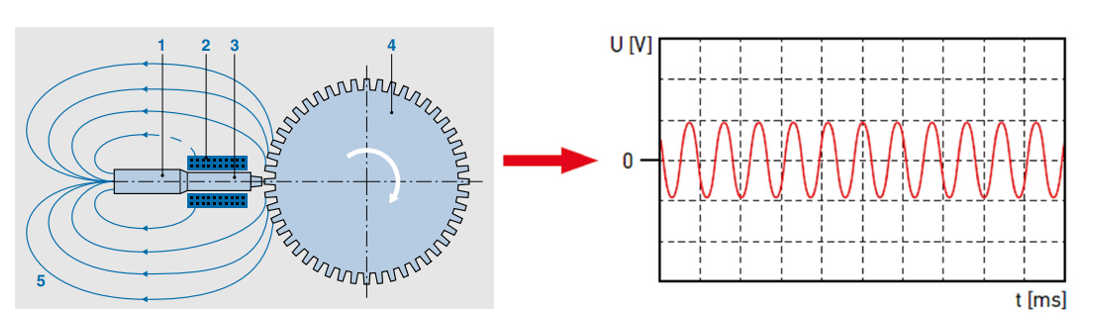
\includegraphics[width=0.8\textwidth]{figuras/diagrama-de-sensor-passivo-e-sinal-gerado.jpg}
    \fonte{ O Autor, adaptado de \cite{Konrad2014}.}
\end{figure}

\subsubsection{Sensor da Roda Modelo Ativo}
\label{sec:metodologia-4-3-2}

Os sensores ativos são usados quase que exclusivamente nos modernos sistemas de freio atuais \cite{Konrad2014}. Esses sensores geralmente consistem em um \gls{CI} circuito integrado hermético de silício de plástico que fica na ponta do sensor(1).  Neste modelo a resistência elétrica muda à medida que o campo magnético muda, e, este comportamento é devido a um anel multipolar(2) usado como uma roda de pulso para sensor. Esses sensores reagem às menores alterações no campo magnético e, portanto, permitem maiores lacunas de ar em comparação com sensores passivos de velocidade da roda, como mostra a Figura~\ref{fig:diagrama-de-sensor-ativo-e-sinal-gerado}.

\begin{figure}[htbp]
    \centering
    \caption{Diagrama de Sensor Ativo e Sinal Gerado.}
    \label{fig:diagrama-de-sensor-ativo-e-sinal-gerado}
    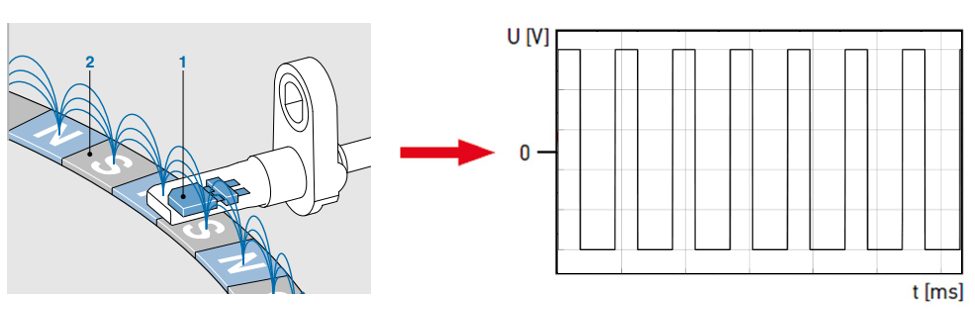
\includegraphics[width=0.8\textwidth]{figuras/diagrama-de-sensor-ativo-e-sinal-gerado.png}
    \fonte{ O Autor, adaptado de \cite{Konrad2014}.}
\end{figure}


\section{Sensor de Pressão de Óleo}
\label{sec:metodologia-5}

O sistema de freio do veículo é complexo e pode concentrar múltiplas válvulas no modulador hidráulico (por exemplo, 12 válvulas em arquiteturas ABS/ESC), sendo que parte delas atua sob alta pressão e diferenciais de pressão elevados (superiores a aproximadamente 0{,}1~MPa, isto é, 1~bar) \cite{Konrad2014}.
Também vale ressaltar que, em estratégias de controle de estabilidade (ESC/ESP), a modulação de pressão de freio por roda é utilizada para contribuir com a estabilidade do veículo por meio de intervenções seletivas de frenagem.

Em veículos com ESC/ESP, é comum a presença de um sensor de pressão para monitorar a pressão hidráulica (por exemplo, associada ao cilindro mestre ou ao circuito), permitindo estimar a ação do condutor e apoiar funções de controle e diagnóstico.

Em aplicações ADAS de controle longitudinal (por exemplo, ACC/AEB), a referência de desaceleração/torque pode ser convertida em uma referência de pressão; quando disponível, a medição de pressão contribui para o fechamento de malha e para a avaliação do desempenho do atuador hidráulico.

\begin{figure}[htbp]
    \centering
    \caption{Sensor de Pressão no Bloco do Sistema de Freio.}
    \label{fig:bloco-do-sistema-de-freio}
    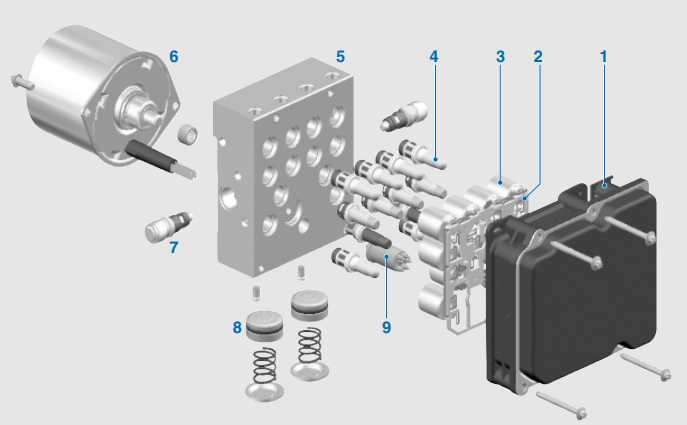
\includegraphics[width=0.8\textwidth]{figuras/bloco-do-sistema-de-freio.jpg}
    \fonte{ O Autor, adaptado de \cite{Konrad2014}.}
\end{figure}

\section{Desenvolvimento da Placa de Controle}
\label{sec:metodologia-6}

O desenvolvimento da placa, tem origem na necessidade de haver um controle das partes relacionadas ao freio, ou seja, o módulo de freio recebe sinais diretamente de sensores ou componentes conectados fisicamente a ele. Isso é mais comum em sistemas críticos que exigem baixa latência ou alta confiabilidade, como sensores de velocidade das rodas, sensores de pressão do freio, e sensores de pedal de freio. 

\begin{figure}[htbp]
    \centering
    \caption{Diagrama em Bloco da Placa Proposta.}
    \label{fig:diagrama-em-bloco-da-placa-proposta}
    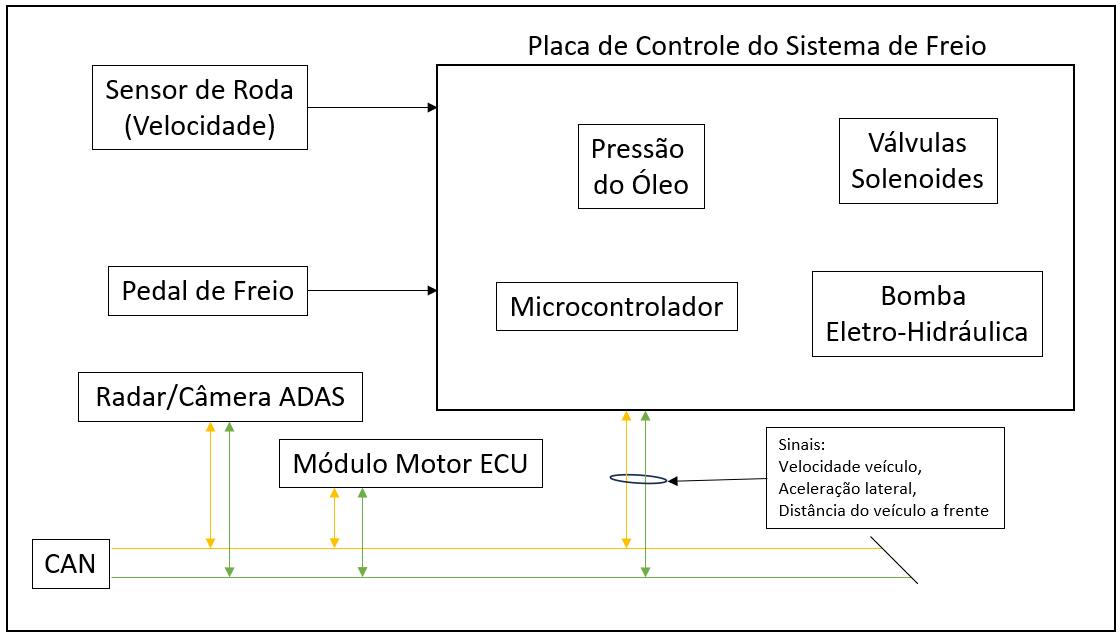
\includegraphics[width=0.8\textwidth]{figuras/diagrama-em-bloco-da-placa-proposta.png}
    \fonte{ O Autor.}
\end{figure}

Também os componentes são controlados para garantir a segurança, estabilidade e eficiência do veículo, como "atuadores de pressão de freio", que controlam a pressão de freio em cada roda; em outras palavras, uma bomba eletro-hidráulica, capaz de gerar pressão de freio independentemente; e ainda, válvulas moduladoras	que regulam a pressão de freio em cada roda e por fim,  um motor de freio de estacionamento, para controlar o freio de estacionamento eletronicamente. A Figura~\ref{fig:diagrama-em-bloco-da-placa-proposta}, apresenta o diagrama em bloco da placa proposta.

\subsection{Circuitos Propostos}
\label{sec:metodologia-6-1}

Os circuitos responsáveis pelo condicionamento de sinais, acionamento de válvulas, controle da bomba e leitura de sensores foram projetados de acordo com os requisitos de baixa latência, compatibilidade elétrica e robustez frente a ruído. 

Cada circuito cumpre uma função específica dentro da plataforma experimental: 
\begin{enumerate}
    \item  condicionamento do sinal do sensor de velocidade,
    \item  acionamento das válvulas solenoides,
    \item  controle do motor da bomba eletro-hidráulica e
    \item  leitura do sensor de pressão.
\end{enumerate}


\begin{comment}
% Comentei essa area, porque nao tinha o appendice referenciado. 
A descrição completa desses circuitos, incluindo seus esquemáticos, diagramas elétricos e simulações, encontra-se no Apêndice~\ref{ap:circuitos-propostos}.


    
\subsection{Circuitos Propostos}
\label{sec:metodologia-6-1}

Para condicionar o sinal proveniente do sensor de velocidade, foi definido um circuito comparador Figura~\ref{fig:circuito-sensor-de-roda-proposto}, uma vez que o sinal pode apresentar ruído e pode ser de uma magnitude baixa, o circuito comparador é ideal neste cenário, por utilizar um amplificador operacional, que possui alta impedância na sua entrada.

Para o condicionamento do sinal proveniente do sensor de velocidade, foi adotado um circuito comparador baseado em amplificador operacional. Esse circuito é responsável por elevar a robustez do sinal e garantir níveis de tensão compatíveis com o microcontrolador utilizado. A descrição completa do circuito, incluindo seu diagrama e análise de funcionamento, encontra-se no Apêndice~\ref{ap:circuito-sensor-roda}.

\begin{figure}[htbp]
    \centering
    \caption{Circuito Sensor de Roda Proposto.}
    \label{fig:circuito-sensor-de-roda-proposto}
    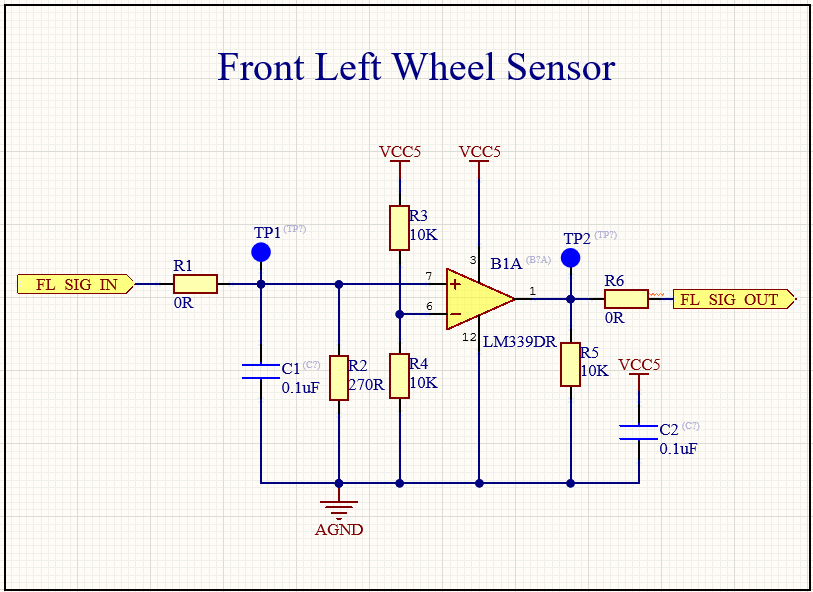
\includegraphics[width=0.8\textwidth]{figuras/circuito-sensor-de-roda-proposto.png}
    \fonte{ O Autor.}
\end{figure}

Foi inserido um comparador que limita a tensão em 2.5V, ou seja, quando o sinal do sensor estiver no ciclo positivo, a saída do amplificar será nível alto lógico, que no caso do microcontrolador escolhido é de 3V3, e quando o sinal do sensor estiver no nível baixo, ou seja, abaixo de 2.5V o sinal será 0V para o microcontrolador, como mostra a simulação do circuito no LTSpice da Figura~\ref{fig:simulacao-circuito-sensor-de-roda-proposto}.

\begin{figure}[htbp]
    \centering
    \caption{Simulação do Circuito Sensor de Roda Proposto.}
    \label{fig:simulacao-circuito-sensor-de-roda-proposto}
    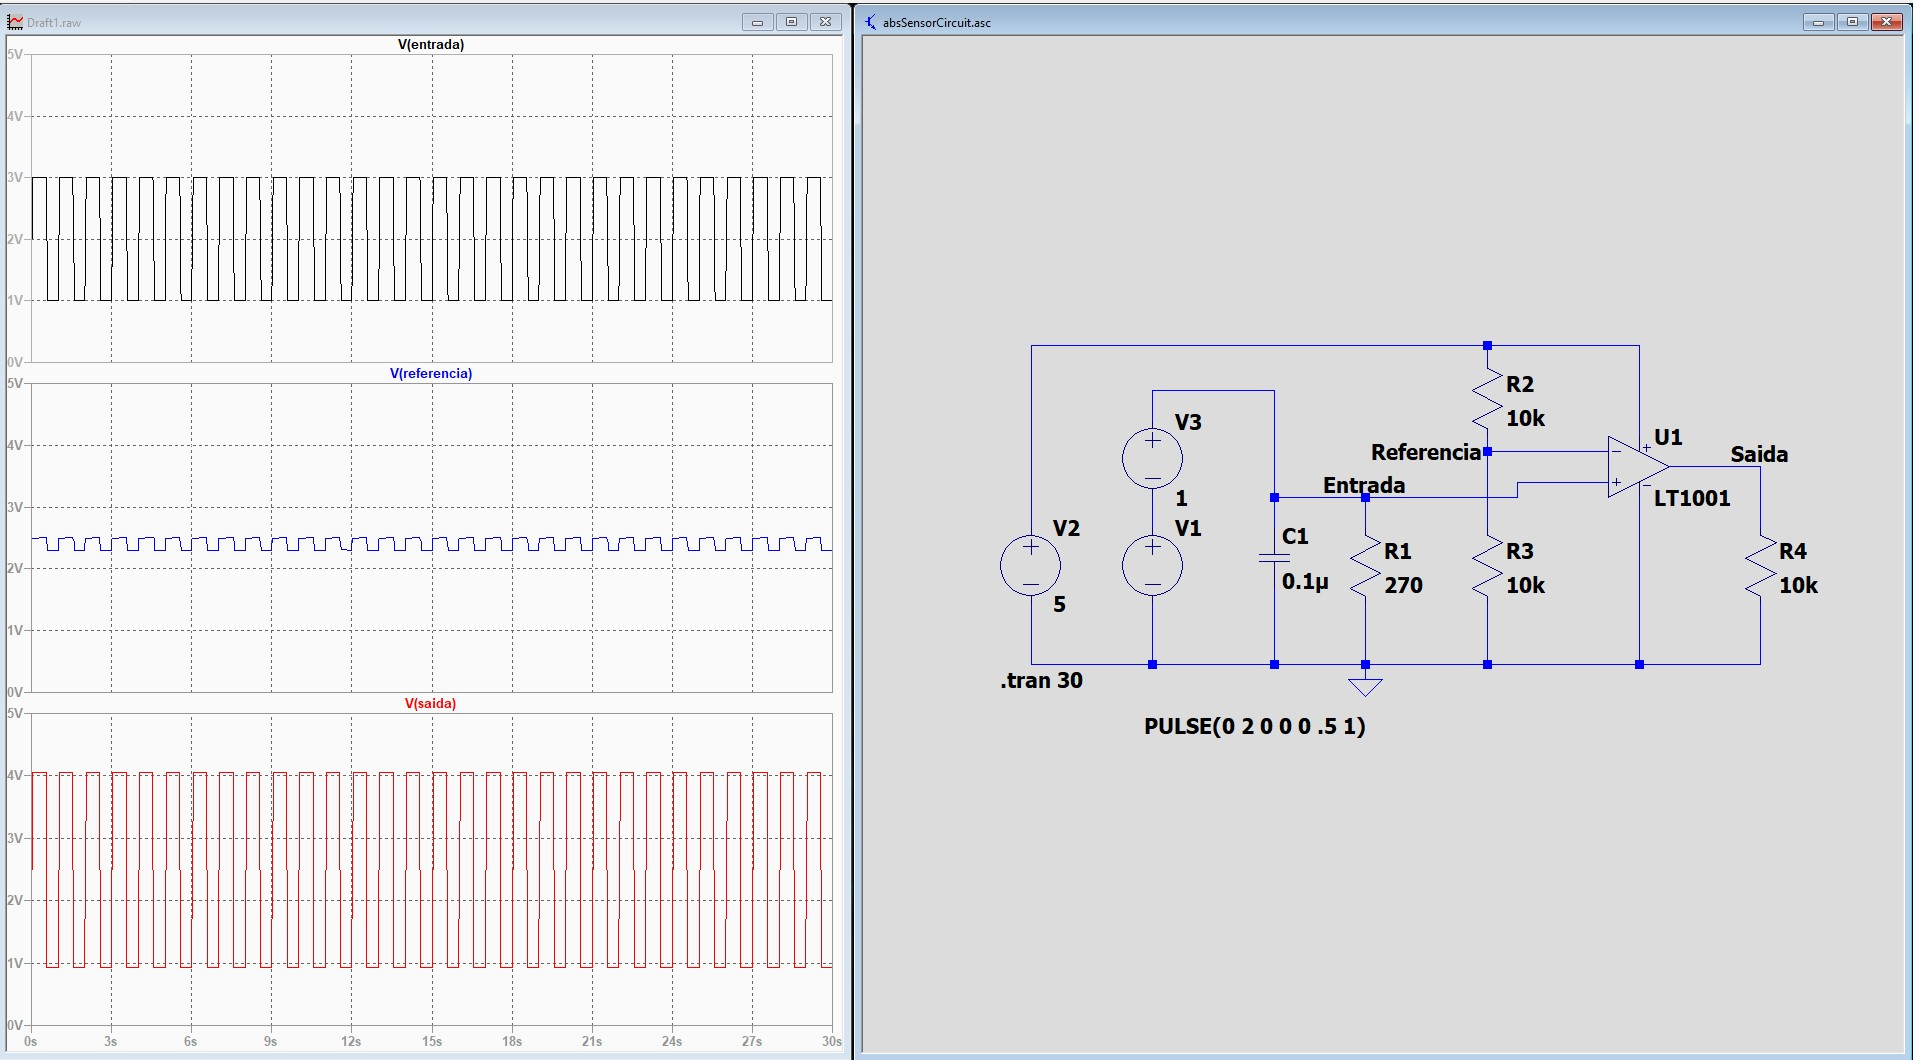
\includegraphics[width=0.8\textwidth]{figuras/simulacao-circuito-sensor-de-roda-proposto.jpg}
    \fonte{ O Autor.}
\end{figure}

\subsection{Circuito da Válvula}
\label{sec:metodologia-6-2}

O circuito da placa, tem como base o kit de Freio da NXP, o KITVALVECNTLEVM \cite{KITVALVECNTLEVM}. Esse kit possui 2 Circuitos Integrados (CI), o MC34SB0800 tem a capacidade de controlar 8 válvulas e um motor, e o MC34SB0410 controla 4 válvulas e um motor. 

O circuito foi totalmente baseado no kit \citeonline{KITVALVECNTLEVM} Figura~\ref{fig:circuito-controle-valvula-solenoide}.
 
\begin{figure}[htbp]
    \centering
    \caption{Circuito de Controle das Válvulas Solenoides.}
    \label{fig:circuito-controle-valvula-solenoide}
    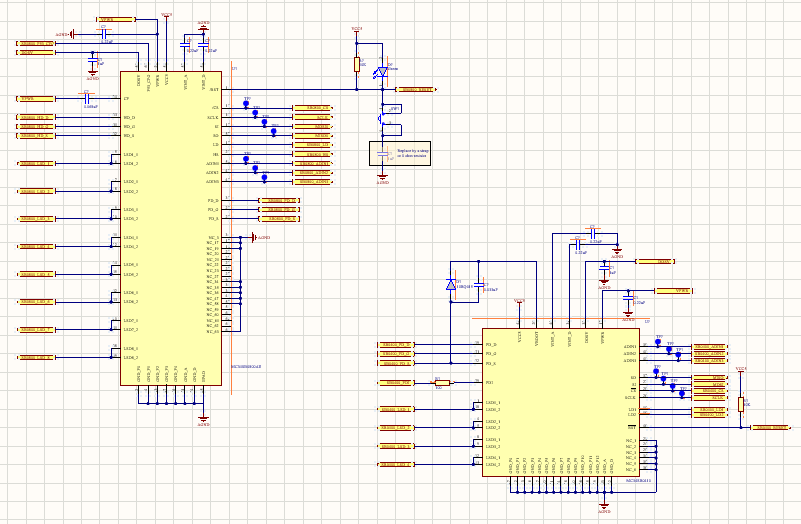
\includegraphics[width=0.8\textwidth]{figuras/circuito-controle-valvula-solenoide.png}
    \fonte{ O Autor adaptado de \cite{MC34SB0800}. }
\end{figure}

\subsection{Circuito da Bomba}
\label{sec:metodologia-6-3}

 O circuito proposto, foi baseado no kit \cite{KITVALVECNTLEVM}, a operação do motor da bomba, se faz ao selecionar o drive de controle, tendo em vista que o MC34SB0800 suporta controle de alta frequência de até 500 Hz \gls{PWM} \cite{MC34SB0800}, enquanto isso, o MC34SB0410 pode lidar com frequências PWM de até 16 kHz, fornecendo operação mais silenciosa e controle mais fino \cite{MC34SB0410}.

Ambos os drives contam com proteções de corrente, para manter a integridade do circuito da Figura~\ref{fig:circuito-controle-valvula-motor}.

\begin{figure}[htbp]
    \centering
    \caption{Circuito de Controle da Bomba de pressão.}
    \label{fig:circuito-controle-valvula-motor}
    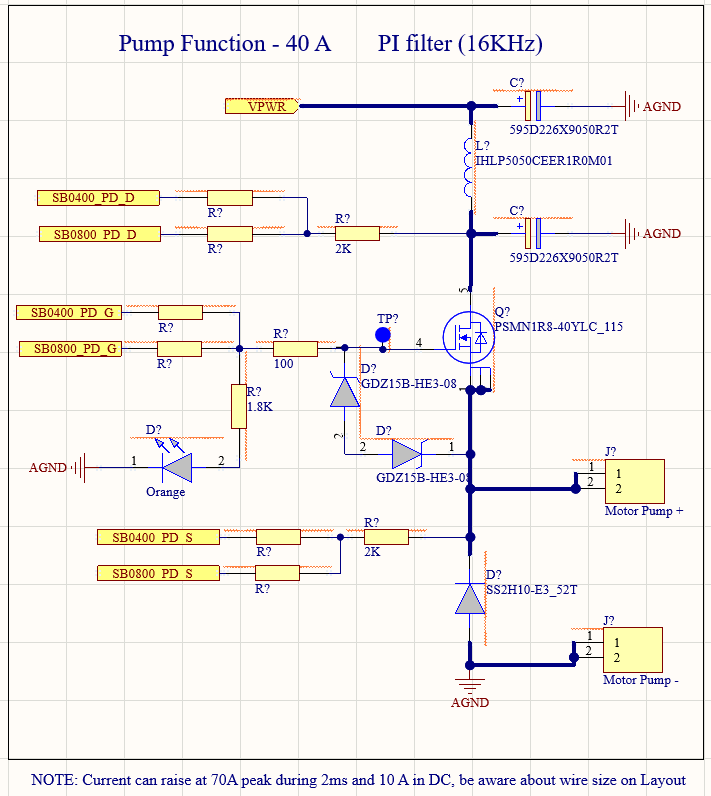
\includegraphics[width=0.8\textwidth]{figuras/circuito-controle-valvula-motor.png}
    \fonte{ O Autor adaptado de \cite{MC34SB0800}. }
\end{figure}

\subsection{Circuito Sensor de Pressão}
\label{sec:metodologia-6-4}

No mercado atual, entre os modelos de sensores encontrados, foram eleitos os sensores piezoresistivos ou tipo \textit{strain gauge}, devido a criticidade desse componente aplicado no sistema de freio, para mitigar uma possível falha de leitura. Também foi decisiva a escolha de circuito de amplificador de instrumentação, por ser menos suscetivo a ruído em seu condicionamento, a Figura~\ref{fig:circuito-sensor-de-pressao-proposto} mostra o circuito para fazer a leitura deste sensor. 

\begin{figure}[htbp]
    \centering
    \caption{Circuito de Leitura do Sensor de Pressão.}
    \label{fig:circuito-sensor-de-pressao-proposto}
    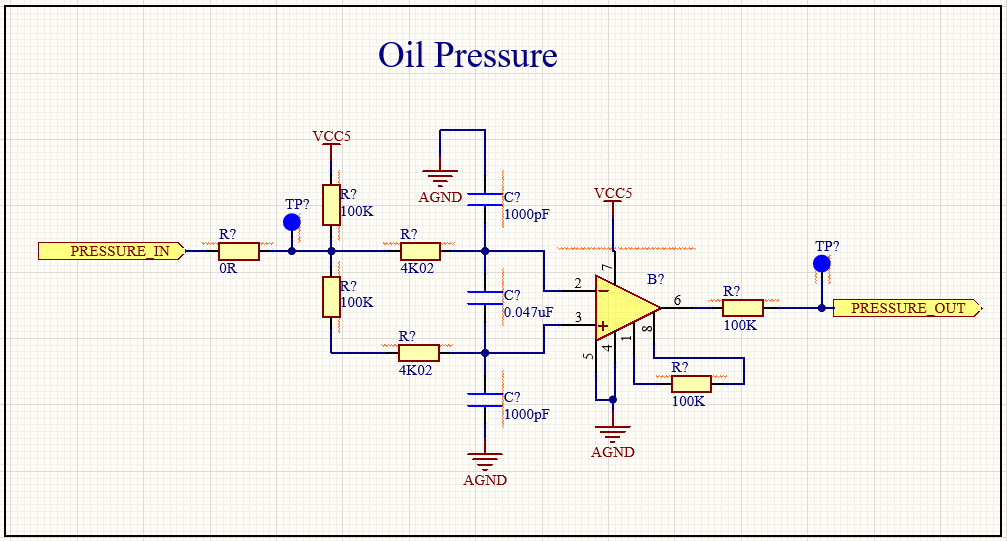
\includegraphics[width=0.8\textwidth]{figuras/circuito-sensor-de-pressao-proposto.png}
    \fonte{ O Autor. }
\end{figure}

\end{comment}

\subsection{Microcontrolador}
\label{sec:metodologia-6-5}

Este projeto tem como base o microcontrolador AURIX TC375 \cite{tc37xDatasheet}, desenvolvido pela empresa \textit{Infineon Technologies}. Corresponde a um microcontrolador multinúcleo para aplicações automotivas devido ao seu alto desempenho; sendo essa uma das principais características, que contribuíram na definição dessa família, além de seu sistema crítico de segurança, ainda mais considerando o campo de frenagem. 
De modo que, abaixo estão elencadas as principais características do microcontrolador AURIX TC375 e, como se encaixa em um sistema de freio em termos de segurança, tecnologia e robustez:

\begin{itemize}
    \item \textbf{Arquitetura multinúcleo:} baseada em CPUs TriCore de 32 bits que operam em sincronia para redundância e tolerância a falhas.
     \item \textbf{Recursos de segurança: } projetado para atender ao mais alto nível de integridade de segurança automotiva (ASIL-D) conforme ISO 26262.
      \item \textbf{Mecanismos de segurança de hardware:} inclui códigos de correção de erros (ECC), unidades de proteção de memória (MPU) e temporizadores \textit{watchdog} para detectar e mitigar falhas.
       \item \textbf{Desempenho:} altas velocidades de \textit{clock} (até 300 MHz) e aceleradores de cálculos complexos, também possui \gls{DSP} (\textit{Digital Signal Processing}) integrados para processamento de sinal em tempo real.
\end{itemize}

Como descrito, este microcontrolador é muito relevante, mas isso não significa que poderia ser empregado unicamente ele na placa, uma vez que, adicionalmente ao microcontrolador AURIX TC375 (INFINEON, 2021), também foi implementada uma conexão na placa visando conectar o Kit de desenvolvimento do TC375\_LITE \cite{tc37xEvaluationBoard}. 

Além disso, uma característica fundamental da placa proposta, é que ela seja flexível quanto ao microcontrolador usado, por esse motivo, foi adicionada uma conexão compatível com Arduino, permitindo desenvolver essa placa com qualquer kit de desenvolvimento desde que com a mesma estrutura.

Durante o desenvolvimento do projeto, o TC375 é responsável pela aquisição dos sinais fornecidos pelo sensor de roda e pelo sensor de pressão. Adicionalmente, uma vez que o kit de desenvolvimento incorpora um \textit{transceiver CAN} baseado no \gls{TLE9251VSJ}, o sistema é capaz de receber informações por meio da rede \gls{CAN}.

A partir de todos os detalhes apresentados, é possível notar que o controle é capaz de definir o exato momento para fazer o acionamento das válvulas e do motor de pressão. 


\subsection{Protocolo de Comunicação CAN}
\label{sec:metodologia-6-6}

 O protocolo \textit{Controller Area Network} (CAN) tem sido amplamente adotado na indústria automotiva e de automação desde sua introdução em 1991 \cite{wiley2022}. Ele proporciona uma comunicação eficiente e confiável entre unidades de controle eletrônico (ECUs), sensores e atuadores, garantindo integridade dos dados e tolerância a falhas. Operando com uma arquitetura multi-mestre, o CAN permite a transmissão de mensagens com base em prioridade, utilizando um sistema de arbitragem que assegura que a mensagem mais importante seja enviada sem colisões. 
 
 A comunicação ocorre por meio de um barramento diferencial de dois fios (CAN\_H e CAN\_L), reduzindo interferências eletromagnéticas e assegurando a robustez da transmissão.
 
 Além disso, o protocolo inclui diversos mecanismos de detecção e correção de erros, como o Cíclico de Redundância (CRC) e a técnica de bit \textit{stuffing}, que garantem a confiabilidade dos dados.
 
 Outrossim, avanços como o \textit{Time-Triggered} CAN (TTCAN) e o CAN com Taxa de Dados Flexível (CAN-FD) ampliaram a aplicabilidade do protocolo, possibilitando transmissões mais rápidas e eficientes, atendendo às exigências dos modernos sistemas automotivos conectados e autônomos.

\section{Demonstração do Funcionamento}
\label{sec:metodologia-7}
Foram realizados testes em simulação para demonstrar o comportamento do sistema e verificar a viabilidade da estratégia de controle no ambiente MATLAB/Simulink. Em paralelo, foi desenvolvido um protótipo de placa eletrônica com foco em viabilizar a futura migração do controlador para execução embarcada e ensaios em bancada.

No escopo deste trabalho, não é apresentada a validação prática do controle em um conjunto físico de freio; essa etapa permanece como continuação natural, conforme discutido no Capítulo~\ref{chap:resultados}.

\section{Descrição dos Instrumentos e Procedimentos}
\label{sec:metodologia-8}
Os instrumentos e ferramentas utilizados incluem o ambiente MATLAB/Simulink para modelagem e simulação, rotinas MATLAB para parametrização e pós-processamento, e a documentação da plataforma eletrônica baseada no microcontrolador AURIX TC375. Os procedimentos incluem: (i) modelagem matemática da planta hidráulica, (ii) implementação do controle digital e da lógica de atuação no Simulink, (iii) registro dos sinais de interesse e (iv) análise dos resultados para diferentes cenários simulados (por exemplo, perfis de referência em patamares e ensaios em malha aberta).

\section{Critérios de Validação}
\label{sec:metodologia-9}
A validação do sistema é conduzida por meio da análise de métricas de desempenho (por exemplo, tempo de subida e de acomodação, sobressinal, erro RMS e erro estacionário), além de inspeção das saturações e do esforço de atuação dos comandos. Essas métricas são calculadas a partir dos sinais registrados no Simulink, conforme detalhado no Capítulo~\ref{chap:resultados}.

Quando aplicável, discute-se a coerência de ordens de grandeza (pressão e vazão) em relação a faixas reportadas na literatura. A conformidade com normas e procedimentos de homologação e a comparação quantitativa com \emph{benchmarks} experimentais ficam fora do escopo deste trabalho.

\section{Simulações: Parâmetros, Modelos e Ferramentas}
\label{sec:metodologia-10}
As simulações foram conduzidas no ambiente MATLAB/Simulink, utilizando modelos matemáticos formulados a partir de equações diferenciais ordinárias e representados no formalismo de espaço de estados. Parâmetros como massa do veículo, pressão hidráulica, frequência de modulação por largura de pulso (PWM) e características dos atuadores foram ajustados visando avaliar o desempenho do sistema sob diferentes condições operacionais.

\section{Desenho Experimental, Amostragem e Análise Estatística}
\label{sec:metodologia-11}
Os ensaios apresentados neste trabalho são baseados em cenários determinísticos de simulação, definidos por perfis de referência e condições de operação do modelo. Dessa forma, a análise é conduzida principalmente por curvas e métricas de desempenho extraídas dos \emph{logs} do Simulink.

Uma avaliação estatística formal (múltiplas execuções com variação sistemática de parâmetros e ruídos, com cálculo de médias e dispersões) é um desdobramento possível para trabalhos futuros, sobretudo em conjunto com validação experimental.

\section{Limitações e Possíveis Vieses}
\label{sec:metodologia-12}
Entre as limitações do estudo, destacam-se restrições do ambiente de simulação, simplificações adotadas nos modelos matemáticos e a ausência de validação do controle em hardware e no conjunto físico de freio. Além disso, ruídos, quantização e atrasos de sensores/atuadores não são explorados de forma exaustiva em todos os cenários.

Como continuidade, recomenda-se a realização de estudos complementares em bancada e/ou em plataformas \textit{hardware-in-the-loop} para validação experimental, conforme discutido na literatura \citeonline{Lv2014}, além de análises de sensibilidade a variações paramétricas e ruídos para consolidar robustez.